%% Journal of Open Research Software Latex template -- Created By Stephen Bonner and John Brennan, Durham Universtiy, UK.

\documentclass{josr}\usepackage[]{graphicx}\usepackage[]{color}
%% maxwidth is the original width if it is less than linewidth
%% otherwise use linewidth (to make sure the graphics do not exceed the margin)
\makeatletter
\def\maxwidth{ %
  \ifdim\Gin@nat@width>\linewidth
    \linewidth
  \else
    \Gin@nat@width
  \fi
}
\makeatother

\definecolor{fgcolor}{rgb}{0.345, 0.345, 0.345}
\newcommand{\hlnum}[1]{\textcolor[rgb]{0.686,0.059,0.569}{#1}}%
\newcommand{\hlstr}[1]{\textcolor[rgb]{0.192,0.494,0.8}{#1}}%
\newcommand{\hlcom}[1]{\textcolor[rgb]{0.678,0.584,0.686}{\textit{#1}}}%
\newcommand{\hlopt}[1]{\textcolor[rgb]{0,0,0}{#1}}%
\newcommand{\hlstd}[1]{\textcolor[rgb]{0.345,0.345,0.345}{#1}}%
\newcommand{\hlkwa}[1]{\textcolor[rgb]{0.161,0.373,0.58}{\textbf{#1}}}%
\newcommand{\hlkwb}[1]{\textcolor[rgb]{0.69,0.353,0.396}{#1}}%
\newcommand{\hlkwc}[1]{\textcolor[rgb]{0.333,0.667,0.333}{#1}}%
\newcommand{\hlkwd}[1]{\textcolor[rgb]{0.737,0.353,0.396}{\textbf{#1}}}%
\let\hlipl\hlkwb

\usepackage{framed}
\makeatletter
\newenvironment{kframe}{%
 \def\at@end@of@kframe{}%
 \ifinner\ifhmode%
  \def\at@end@of@kframe{\end{minipage}}%
  \begin{minipage}{\columnwidth}%
 \fi\fi%
 \def\FrameCommand##1{\hskip\@totalleftmargin \hskip-\fboxsep
 \colorbox{shadecolor}{##1}\hskip-\fboxsep
     % There is no \\@totalrightmargin, so:
     \hskip-\linewidth \hskip-\@totalleftmargin \hskip\columnwidth}%
 \MakeFramed {\advance\hsize-\width
   \@totalleftmargin\z@ \linewidth\hsize
   \@setminipage}}%
 {\par\unskip\endMakeFramed%
 \at@end@of@kframe}
\makeatother

\definecolor{shadecolor}{rgb}{.97, .97, .97}
\definecolor{messagecolor}{rgb}{0, 0, 0}
\definecolor{warningcolor}{rgb}{1, 0, 1}
\definecolor{errorcolor}{rgb}{1, 0, 0}
\newenvironment{knitrout}{}{} % an empty environment to be redefined in TeX

\usepackage{alltt}



%% revised text
\newcommand{\new}[1]{{\color{blue} #1}}

%% packages
\usepackage{natbib}

\usepackage{subfig}
\usepackage{amsmath}
\usepackage{tikz}
\usetikzlibrary{shapes,arrows,positioning}

\usepackage{booktabs}

%% Nice inline code
\makeatletter
\newcommand*{\textalltt}{}
\DeclareRobustCommand*{\textalltt}{%
  \begingroup
    \let\do\@makeother
    \dospecials
    \catcode`\\=\z@
    \catcode`\{=\@ne
    \catcode`\}=\tw@
    \verbatim@font\@noligs
    \@vobeyspaces
    \frenchspacing
    \@textalltt
}
\newcommand*{\@textalltt}[1]{%
    #1%
  \endgroup
}
\makeatother


%% Set the header information
\pagestyle{fancy}
\definecolor{mygray}{gray}{0.6}
\renewcommand\headrule{}
\rhead{\footnotesize 3}
\rhead{\textcolor{gray}{UP JORS software Latex paper template version 0.1}}
\IfFileExists{upquote.sty}{\usepackage{upquote}}{}
\begin{document}
\hypersetup{pageanchor=false}





{\bf Software paper for submission to the Journal of Open Research Software} \\

%To complete this template, please replace the blue text with your own. The paper has three main sections: (1) Overview; (2) Availability; (3) Reuse potential. \\

%Please submit the completed paper to: editor.jors@ubiquitypress.com

\rule{\textwidth}{1pt}

\section*{(1) Overview}

\vspace{0.5cm}

\section*{Title}
model4you: An R package for personalised treatment effect estimation


\section*{Paper Authors}
1. Seibold, Heidi; 2. Zeileis, Achim; 3. Hothorn, Torsten



\section*{Paper Author Roles and Affiliations}
1. \new{Postdoc; Institute for Medical
Information Processing, Biometry, and Epidemiology, LMU Munich}

2. Professor; Department of Statistics, Faculty of Economics and Statistics,
University of Innsbruck

3. Professor; Biostatistics Department, Epidemiology, Biostatistics \&
Prevention Institute, University of Zurich



\section*{Abstract}
Typical models estimating treatment effects assume that the treatment effect is
the same for all individuals.  Model-based recursive partitioning allows to
relax this assumption and to estimate stratified treatment effects (model-based
trees) or even personalised treatment effects (model-based forests).  With
model-based trees one can compute treatment effects for different strata of
individuals. The strata are found in a data-driven fashion and depend on
characteristics of the individuals.  Model-based random forests allow for a
similarity estimation between individuals in terms of model parameters (e.g.~
intercept and treatment effect). The similarity measure can then be used to
estimate personalised models.  The R package \emph{model4you} implements these
stratified and personalised models \new{in the setting with two randomly
assigned treatments} with a focus on ease of use and interpretability so that
clinicians and other users can take the model they usually use for the
estimation of the average treatment effect and with a few lines of code get a
visualisation that is easy to understand and interpret.

%\textcolor{blue}{A short (ca. 100 word) summary of the software being described: what problem the software addresses, how it was implemented and architected, where it is stored, and its reuse potential.}

\section*{Keywords}

personalised medicine; subgroup analysis; model-based recursive partitioning;
unbiased trees; treatment effect; random forest


\section*{Introduction}

%\textcolor{blue}{An overview of the software, how it was produced, and the research for which it has been used, including references to relevant research articles. A short comparison with software which implements similar functionality should be included in this section. }
Studies in various fields randomly assign individuals to one of two groups with
different exposure and then measure a response. For example, in clinical trials
patients are assigned to one of two treatment groups where usually one
treatment group receives a new treatment or drug and the other treatment group
receives the standard of care or a placebo. Other examples are in A-B testing
in marketing studies or any other two group comparisons such as the mathematics
exam discussed below, where students were divided into different exam groups
and received slightly different exam tasks. In the following we will refer to
the two groups as \emph{treatment groups} and to the group indicator as
\emph{treatment indicator}, which always takes values $0$ (individual in first
group) and $1$ (individual in second group).

Treatment effect estimation is often done using simple models with the binary
treatment indicator as only covariate. In the example of a clinical trial the
treatment indicator would be $1$ if the patient receives the new treatment and
$0$ if the patient receives standard of care.  In R such a simple model can be
estimated as follows:
\begin{knitrout}
\definecolor{shadecolor}{rgb}{0.969, 0.969, 0.969}\color{fgcolor}\begin{kframe}
\begin{alltt}
\hlstd{base_model} \hlkwb{<-} \hlkwd{model}\hlstd{(response} \hlopt{~} \hlstd{treatment, data)}
\end{alltt}
\end{kframe}
\end{knitrout}
with \texttt{\hlstd{response}} being the response measured, \texttt{\hlstd{treatment}} being
the treatment indicator and \texttt{\hlstd{data}} being the data set containing these
variables.  The function \texttt{\hlkwd{model}\hlstd{()}} can be replaced for example by
\texttt{\hlkwd{lm}\hlstd{()}} to estimate a linear model, \texttt{\hlkwd{glm}\hlstd{()}} to estimate a
generalised linear model or \texttt{\hlkwd{survreg}\hlstd{()}} to estimate a parametric
survival model.  These models estimate intercept and treatment effect for all
individuals in the \texttt{\hlstd{data}} and allow for predicting the response of
other individuals given they do or do not receive the treatment of interest.

For cases where the assumption that all individuals have the same intercept and
treatment effect is too strict the R package \emph{model4you} offers two
options:

\paragraph{1. Model-based trees} identify subgroups where within the subgroups
the model parameters are similar and between groups the model parameters are
different. This is achieved by finding instabilities in the model parameters
with respect to a variable (characteristic) and recursively partitioning the
data into groups. If, for example the algorithm finds that men and women have
differing treatment effects, the data are partitioned into two subgroups.
Details on model-based trees in general can be found in
\citep{zeileis_model-based_2008} and for the special use case for stratified
treatment effect estimation in \citep{seibold_model-based_2016}.  Just a single
line of code lets the user compute a model-based tree in R:
\begin{knitrout}
\definecolor{shadecolor}{rgb}{0.969, 0.969, 0.969}\color{fgcolor}\begin{kframe}
\begin{alltt}
\hlstd{strat_models} \hlkwb{<-} \hlkwd{pmtree}\hlstd{(base_model)}
\end{alltt}
\end{kframe}
\end{knitrout}
Note that \texttt{\hlkwd{pmtree}\hlstd{()}} uses the data given in the call of the base model.
It automatically uses variables not used in the model formula (in the example
above \texttt{\hlstd{response} \textalltt{~} \hlstd{treatment}}) as potential subgroup defining variables.
This can be edited using the \texttt{\hlstd{zformula}} argument.

\paragraph{2. Personalised models} use model-based random forests to estimate
similarity of individuals in terms of model parameters. For each individual a
personalised model can be estimated based on a weighted set of the original
data, where the similarity measure corresponds to the weight. Details on the
personalised models can be found in \citep{seibold_individual_2017}.  Computing
personalised models for all observations in the training data is simple:
\begin{knitrout}
\definecolor{shadecolor}{rgb}{0.969, 0.969, 0.969}\color{fgcolor}\begin{kframe}
\begin{alltt}
\hlstd{pm_forest} \hlkwb{<-} \hlkwd{pmforest}\hlstd{(base_model)}
\hlstd{pers_models} \hlkwb{<-} \hlkwd{pmodel}\hlstd{(pm_forest)}
\end{alltt}
\end{kframe}
\end{knitrout}
Again here the potential effect-modifying variables are taken by default as all
variables not given in the model formula and can be defined using the
\texttt{\hlstd{zformula}} argument in \texttt{\hlkwd{pmforest}\hlstd{()}}.


In the following we will present an example application for model-based trees
and personalised models. For this we need to load the package and -- to ensure
reproducibility -- set a random seed.
\new{
Also for visualisations we need packages
\emph{ggplot2} \citep{ggplot2}, \emph{ggbeeswarm} \citep{ggbeeswarm} and
\emph{gridExtra} \citep{gridExtra}. The data used is
available in the \emph{psychotools} package \citep{psychotools}.
}
\begin{knitrout}
\definecolor{shadecolor}{rgb}{0.969, 0.969, 0.969}\color{fgcolor}\begin{kframe}
\begin{alltt}
\hlkwd{library}\hlstd{(}\hlstr{"model4you"}\hlstd{)}
\hlkwd{set.seed}\hlstd{(}\hlnum{2017}\hlstd{)}

\hlkwd{library}\hlstd{(}\hlstr{"ggplot2"}\hlstd{)}
\hlkwd{theme_set}\hlstd{(}\hlkwd{theme_classic}\hlstd{())}
\hlkwd{library}\hlstd{(}\hlstr{"ggbeeswarm"}\hlstd{)}
\hlkwd{library}\hlstd{(}\hlstr{"gridExtra"}\hlstd{)}
\end{alltt}
\end{kframe}
\end{knitrout}

\paragraph{Mathematics exam analysis:}
In 2014 first-year business and economics students at the University of
Innsbruck were divided into two examination groups. Group 1 took the exam in
the morning and group 2 started after the first group finished. The exams for
the two groups were slightly different.  The data can be accessed and prepared
as follows:

\begin{knitrout}
\definecolor{shadecolor}{rgb}{0.969, 0.969, 0.969}\color{fgcolor}\begin{kframe}
\begin{alltt}
\hlkwd{data}\hlstd{(}\hlstr{"MathExam14W"}\hlstd{,} \hlkwc{package} \hlstd{=} \hlstr{"psychotools"}\hlstd{)}

\hlcom{## scale points achieved to [0, 100] percent}
\hlstd{MathExam14W}\hlopt{$}\hlstd{tests} \hlkwb{<-} \hlnum{100} \hlopt{*} \hlstd{MathExam14W}\hlopt{$}\hlstd{tests}\hlopt{/}\hlnum{26}
\hlstd{MathExam14W}\hlopt{$}\hlstd{pcorrect} \hlkwb{<-} \hlnum{100} \hlopt{*} \hlstd{MathExam14W}\hlopt{$}\hlstd{nsolved}\hlopt{/}\hlnum{13}

\hlcom{## select variables to be used}
\hlstd{MathExam} \hlkwb{<-} \hlstd{MathExam14W[ ,} \hlkwd{c}\hlstd{(}\hlstr{"pcorrect"}\hlstd{,} \hlstr{"group"}\hlstd{,} \hlstr{"tests"}\hlstd{,} \hlstr{"study"}\hlstd{,}
                             \hlstr{"attempt"}\hlstd{,} \hlstr{"semester"}\hlstd{,} \hlstr{"gender"}\hlstd{)]}
\end{alltt}
\end{kframe}
\end{knitrout}
\new{To investigate the correlation between exam group and exam performance, we
compute a simple linear model regressing the percentage points of correct
answers on the exam group.}
\begin{knitrout}
\definecolor{shadecolor}{rgb}{0.969, 0.969, 0.969}\color{fgcolor}\begin{kframe}
\begin{alltt}
\hlstd{bmod_math} \hlkwb{<-} \hlkwd{lm}\hlstd{(pcorrect} \hlopt{~} \hlstd{group,} \hlkwc{data} \hlstd{= MathExam)}
\end{alltt}
\end{kframe}
\end{knitrout}
The estimates and confidence intervals of this model can be computed via
\begin{knitrout}
\definecolor{shadecolor}{rgb}{0.969, 0.969, 0.969}\color{fgcolor}\begin{kframe}
\begin{alltt}
\hlkwd{cbind}\hlstd{(}\hlkwc{estimate} \hlstd{=} \hlkwd{coef}\hlstd{(bmod_math),} \hlkwd{confint}\hlstd{(bmod_math))}
\end{alltt}
\begin{verbatim}
##              estimate     2.5 %   97.5 %
## (Intercept) 57.600184 55.122708 60.07766
## group2      -2.332414 -5.698108  1.03328
\end{verbatim}
\end{kframe}
\end{knitrout}
The model can be visualised by plotting the estimated densities
(see Figure~\ref{fig:math_bmod_vis}):
\begin{knitrout}
\definecolor{shadecolor}{rgb}{0.969, 0.969, 0.969}\color{fgcolor}\begin{kframe}
\begin{alltt}
\hlkwd{lm_plot}\hlstd{(bmod_math)}
\end{alltt}
\end{kframe}\begin{figure}

{\centering 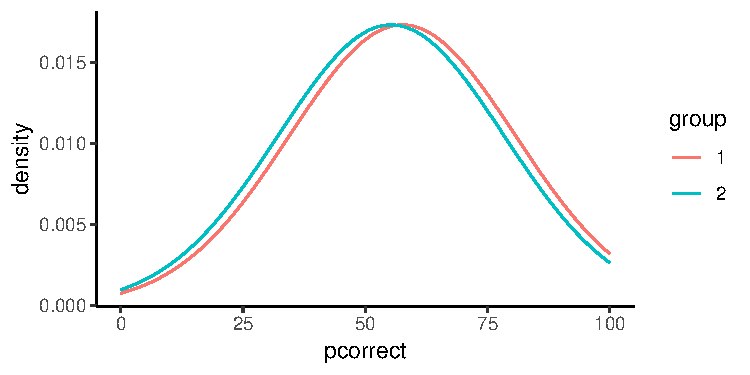
\includegraphics[width=0.7\textwidth]{figure/math_bmod_vis-1} 

}

\caption[Density estimates of base model for the Mathematics Exam data]{Density estimates of base model for the Mathematics Exam data.}\label{fig:math_bmod_vis}
\end{figure}


\end{knitrout}
Both the estimates and confidence intervals and the density curves suggest that
there is almost no difference between the two groups. But does this really hold
for all types of students?

A tree based on this model can be computed and visualised in only two lines of
code:
\begin{knitrout}
\definecolor{shadecolor}{rgb}{0.969, 0.969, 0.969}\color{fgcolor}\begin{kframe}
\begin{alltt}
\hlstd{tr_math} \hlkwb{<-} \hlkwd{pmtree}\hlstd{(bmod_math,} \hlkwc{control} \hlstd{=} \hlkwd{ctree_control}\hlstd{(}\hlkwc{maxdepth} \hlstd{=} \hlnum{2}\hlstd{))}
\hlkwd{plot}\hlstd{(tr_math,} \hlkwc{terminal_panel} \hlstd{=} \hlkwd{node_pmterminal}\hlstd{(tr_math,}
                                               \hlkwc{plotfun} \hlstd{= lm_plot))}
\end{alltt}
\end{kframe}\begin{figure}

{\centering 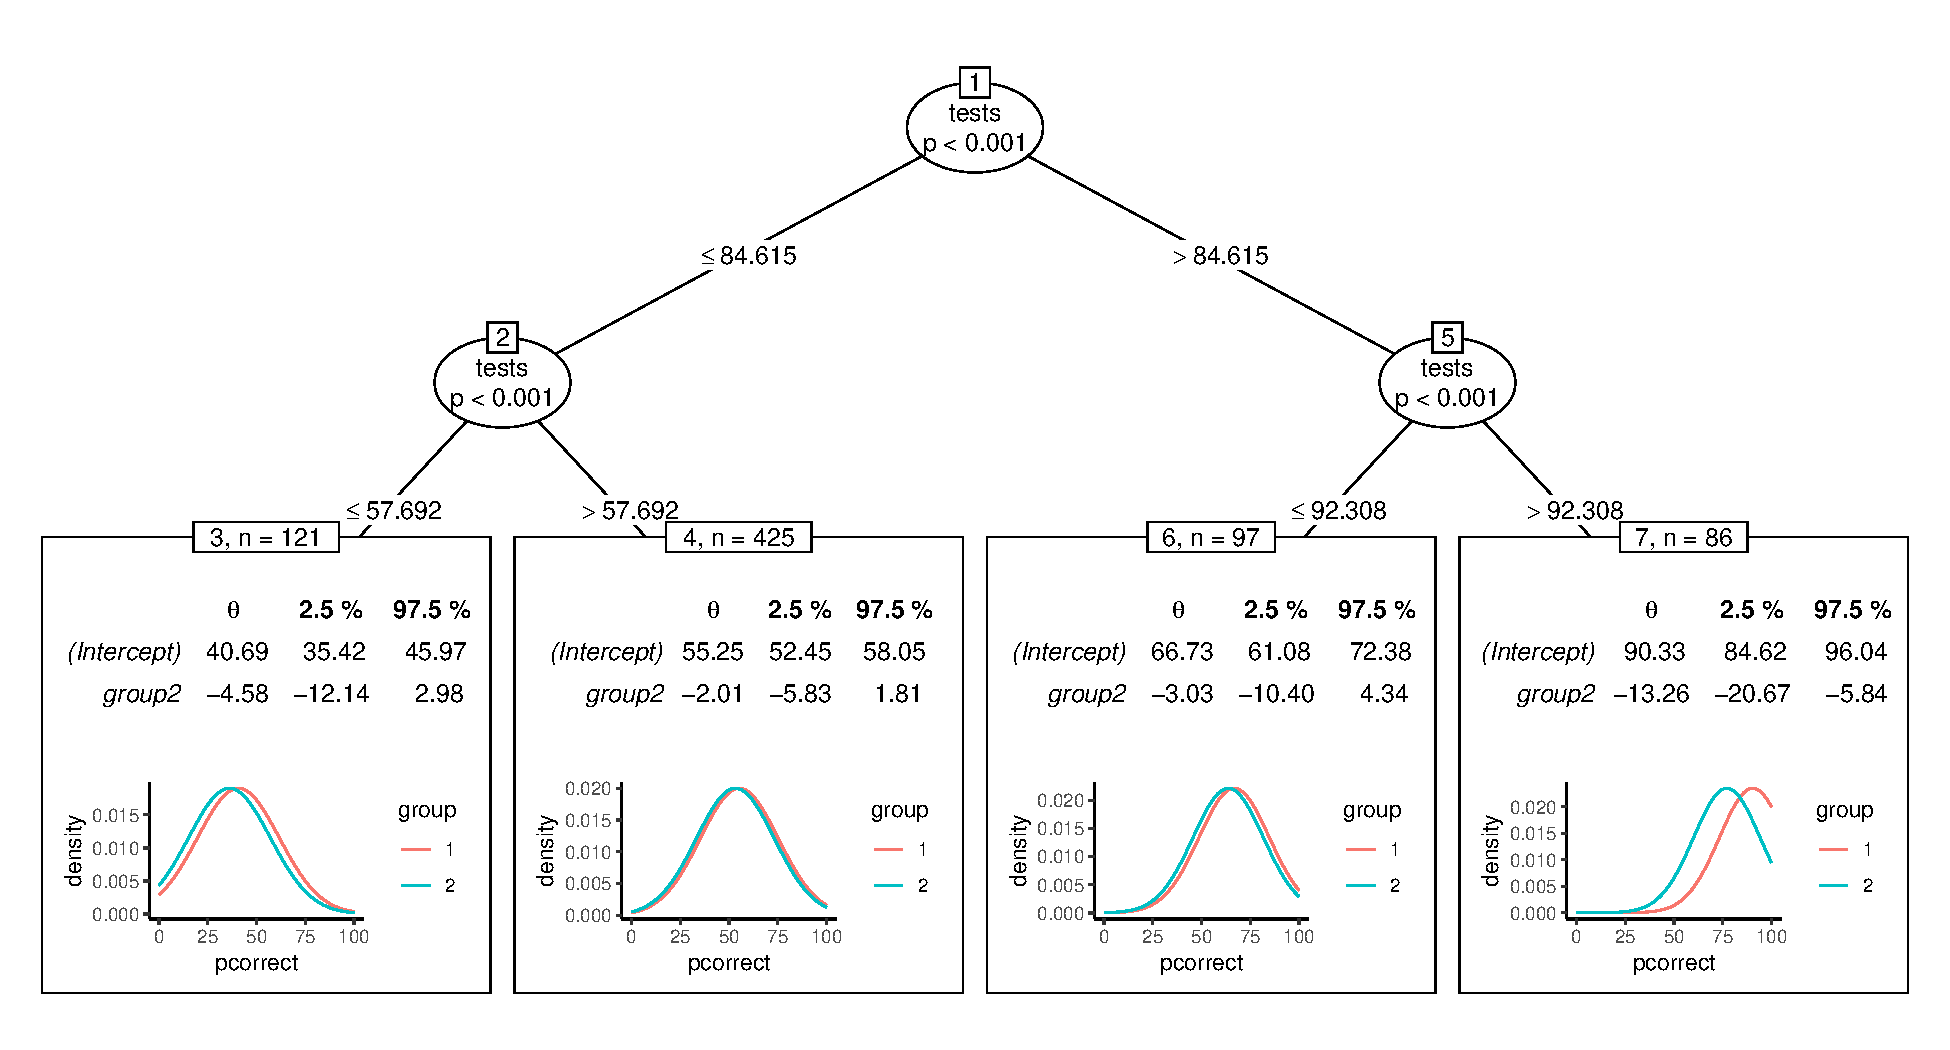
\includegraphics[width=\maxwidth]{figure/math_tree-1} 

}

\caption[Personalised model tree for the Mathematics Exam datam]{Personalised model tree for the Mathematics Exam datam.}\label{fig:math_tree}
\end{figure}


\end{knitrout}
\new{
We restrict the depth of the tree to two (\texttt{\hlstd{maxdepth} \hlkwb{=} \hlnum{2}}) for
illustration purposes. If this setting is not used a more complex tree would be
estimated. Also the cutpoints and effect estimates are rounded in the plot.  To
view the tree in the R console, the \texttt{\hlkwd{print}\hlstd{()}} function can be
used.
}
\begin{knitrout}
\definecolor{shadecolor}{rgb}{0.969, 0.969, 0.969}\color{fgcolor}\begin{kframe}
\begin{alltt}
\hlkwd{print}\hlstd{(tr_math)}
\end{alltt}
\begin{verbatim}
## [1] root
## |   [2] tests <= 84.61538
## |   |   [3] tests <= 57.69231: n = 121
## |   |       (Intercept)      group2 
## |   |         40.694789   -4.580056 
## |   |   [4] tests > 57.69231: n = 425
## |   |       (Intercept)      group2 
## |   |         55.251855   -2.012988 
## |   [5] tests > 84.61538
## |   |   [6] tests <= 92.30769: n = 97
## |   |       (Intercept)      group2 
## |   |         66.730769   -3.033063 
## |   |   [7] tests > 92.30769: n = 86
## |   |       (Intercept)      group2 
## |   |          90.32967   -13.25576 
## 
## Number of inner nodes:    3
## Number of terminal nodes: 4
## Number of parameters per node: 2
## Objective function: -276167.6
\end{verbatim}
\end{kframe}
\end{knitrout}
The tree (see Figure~\ref{fig:math_tree}) divides students based on the
percentage of successful online \texttt{\hlstd{tests}}. These online tests were
conducted biweekly throughout the semester.  The largest difference between the
two exam groups is in the students who did very well in the online tests (more
than \texttt{92.3} percent correct). The
tree thus gives us much more information on the fairness of the exam than the
simple linear model, which is that it does not seem to be fair for students who
did very well throughout the semester (at this point we should state that the
students self selected into the two exam groups which might also be the reason
for differences in exam performance).
\new{Note that confidence intervals shown in the tree are not adjusted for
selection of the cutpoints in the tree and
should hence be interpreted as a measure for variablity and not be used for
inference.}

Estimating personalised models is almost as simple as the stratified models:
\begin{knitrout}
\definecolor{shadecolor}{rgb}{0.969, 0.969, 0.969}\color{fgcolor}\begin{kframe}
\begin{alltt}
\hlstd{forest_math} \hlkwb{<-} \hlkwd{pmforest}\hlstd{(bmod_math)}
\hlstd{pmods_math} \hlkwb{<-} \hlkwd{pmodel}\hlstd{(forest_math)}

\hlcom{## model parameters of first 6 students}
\hlkwd{head}\hlstd{(pmods_math)}
\end{alltt}
\begin{verbatim}
##   (Intercept)     group2
## 1    54.07712 -10.044714
## 2    40.17963  -6.326631
## 3    49.95619  -6.782954
## 4    53.19826  -9.367226
## 5    64.00692  -4.593500
## 6    41.13722  -6.465630
\end{verbatim}
\end{kframe}
\end{knitrout}

Dependence plots with the group effect (treatment effect) on the y-axis and
the student characteristics on the x-axis are a good way of visualising the
personalised models and for getting knowledge about the interactions between
student characteristics and the exam group.
\new{
Note that the plot is related to but not the same as the classical partial
dependence plot \citep{friedman2001greedy}, as each point in the figure is one
patient in the given data set.  Since the percentage of successful online tests
is measured on a grid, a beeswarm plot (a variant of jittered scatter plot)
possibly shows the relationships even better than the scatter plot (both shown
in Figure~\ref{fig:math_dp1}, Figure~\ref{fig:math_dp11} includes a loess
curve). We see a nonlinear relation between the percentage of successful online
\texttt{\hlstd{tests}} and the exam group effect. Students with great
performance during the semenster are estimated to have the strongest effect.
}
\begin{knitrout}
\definecolor{shadecolor}{rgb}{0.969, 0.969, 0.969}\color{fgcolor}\begin{kframe}
\begin{alltt}
\hlstd{dpdat_math} \hlkwb{<-} \hlkwd{cbind}\hlstd{(pmods_math, MathExam)}

\hlkwd{ggplot}\hlstd{(dpdat_math,} \hlkwd{aes}\hlstd{(}\hlkwc{x} \hlstd{= tests,} \hlkwc{y} \hlstd{= group2))} \hlopt{+}
  \hlkwd{geom_point}\hlstd{(}\hlkwc{alpha} \hlstd{=} \hlnum{0.2}\hlstd{,} \hlkwc{size} \hlstd{=} \hlnum{1}\hlstd{)} \hlopt{+}
  \hlkwd{geom_smooth}\hlstd{(}\hlkwc{fill} \hlstd{=} \hlnum{NA}\hlstd{,} \hlkwc{method} \hlstd{=} \hlstr{"loess"}\hlstd{)} \hlopt{+}
  \hlkwd{theme}\hlstd{(}\hlkwc{legend.position} \hlstd{=} \hlstr{"none"}\hlstd{)} \hlopt{+}
  \hlkwd{ylab}\hlstd{(}\hlstr{"estimated individual\textbackslash{}nexam group effect"}\hlstd{)}

\hlkwd{ggplot}\hlstd{(dpdat_math,} \hlkwd{aes}\hlstd{(}\hlkwc{x} \hlstd{= tests,} \hlkwc{y} \hlstd{= group2,} \hlkwc{color} \hlstd{= tests))} \hlopt{+}
  \hlkwd{geom_quasirandom}\hlstd{(}\hlkwc{alpha} \hlstd{=} \hlnum{0.5}\hlstd{,} \hlkwc{size} \hlstd{=} \hlnum{1}\hlstd{)} \hlopt{+}
  \hlkwd{theme}\hlstd{(}\hlkwc{legend.position} \hlstd{=} \hlstr{"none"}\hlstd{)} \hlopt{+}
  \hlkwd{ylab}\hlstd{(}\hlstr{"estimated individual\textbackslash{}nexam group effect"}\hlstd{)}
\end{alltt}
\end{kframe}\begin{figure}

{\centering \subfloat[Scatter plot with loess curve.\label{fig:math_dp11}]{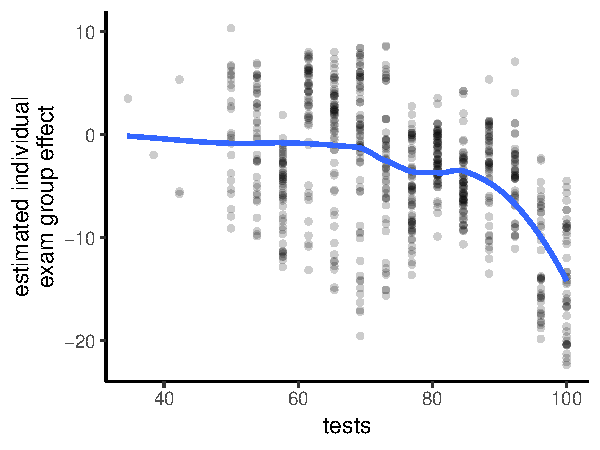
\includegraphics[width=.48\linewidth]{figure/math_dp1-1} }
\subfloat[Beeswarm plot.\label{fig:math_dp12}]{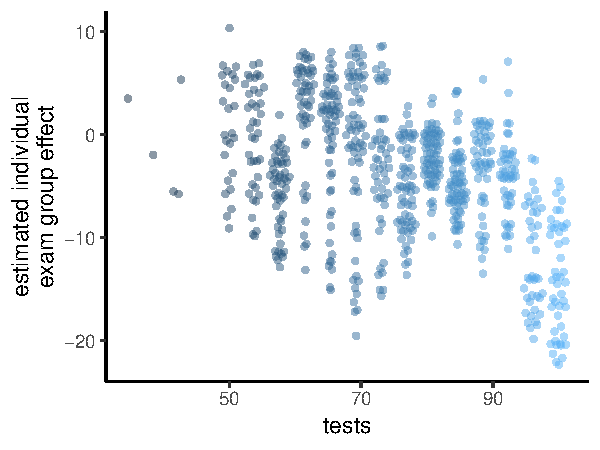
\includegraphics[width=.48\linewidth]{figure/math_dp1-2} }

}

\caption[Dependence plot for percentage of tests successfully solved]{Dependence plot for percentage of tests successfully solved.}\label{fig:math_dp1}
\end{figure}


\end{knitrout}

\new{
For categorical variables such as the number of previous attempts to pass the
exam (\texttt{\hlstd{attempt}}) and \texttt{\hlstd{gender}} we can use box plots,
\new{beeswarm} plots or a combination thereof (as in
Figure~\ref{fig:math_dp21}). Figure~\ref{fig:math_dp22} shows the number of
previous attempts on the x-axis and the color indicates the gender of each
student.  This way we can see that for students writing the exam for the first
time, gender seems to play a bigger role in terms of estimated individual exam
group effect than for others.
}
\begin{knitrout}
\definecolor{shadecolor}{rgb}{0.969, 0.969, 0.969}\color{fgcolor}\begin{kframe}
\begin{alltt}
\hlkwd{ggplot}\hlstd{(dpdat_math,} \hlkwd{aes}\hlstd{(}\hlkwc{x} \hlstd{= gender,} \hlkwc{y} \hlstd{= group2,} \hlkwc{color} \hlstd{= gender))} \hlopt{+}
  \hlkwd{geom_boxplot}\hlstd{()} \hlopt{+}
  \hlkwd{geom_quasirandom}\hlstd{(}\hlkwc{alpha} \hlstd{=} \hlnum{0.5}\hlstd{)} \hlopt{+}
  \hlkwd{theme}\hlstd{(}\hlkwc{legend.position} \hlstd{=} \hlstr{"none"}\hlstd{)} \hlopt{+}
  \hlkwd{ylab}\hlstd{(}\hlstr{"estimated individual\textbackslash{}nexam group effect"}\hlstd{)}

\hlkwd{ggplot}\hlstd{(dpdat_math,} \hlkwd{aes}\hlstd{(}\hlkwc{x} \hlstd{= attempt,} \hlkwc{y} \hlstd{= group2,} \hlkwc{color} \hlstd{= gender))} \hlopt{+}
  \hlkwd{geom_quasirandom}\hlstd{(}\hlkwc{alpha} \hlstd{=} \hlnum{0.5}\hlstd{)} \hlopt{+}
  \hlkwd{ylab}\hlstd{(}\hlstr{"estimated individual\textbackslash{}nexam group effect"}\hlstd{)}
\end{alltt}
\end{kframe}\begin{figure}

{\centering \subfloat[Gender.\label{fig:math_dp21}]{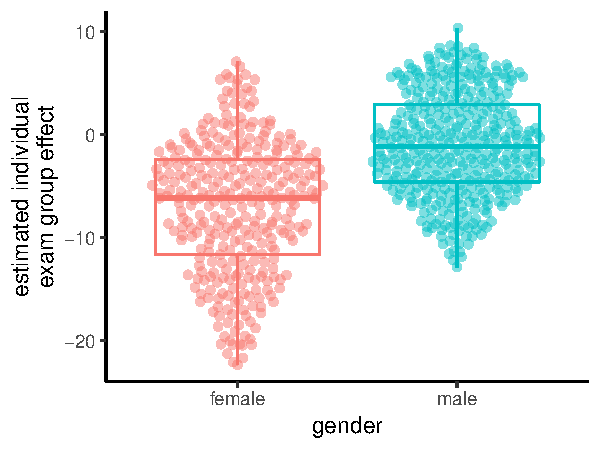
\includegraphics[width=.48\linewidth]{figure/math_dp2-1} }
\subfloat[Number of previous attempts and gender.\label{fig:math_dp22}]{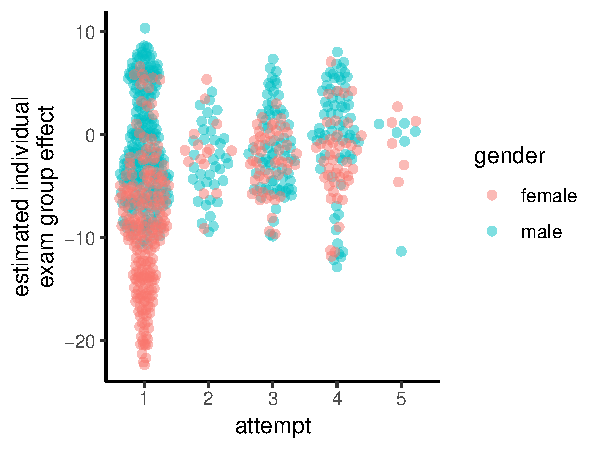
\includegraphics[width=.48\linewidth]{figure/math_dp2-2} }

}

\caption[Dependence plots for the number of previous attempts and gender]{Dependence plots for the number of previous attempts and gender.}\label{fig:math_dp2}
\end{figure}


\end{knitrout}

With the tools provided by the \emph{model4you} package it is very
simple to create understandable stratified and personalised models
and compelling visualisations that can be used to communicate these
models.



\section*{Implementation and architecture}
The R package \emph{model4you} is focused on ease of use and
interpretability.  Users can take a simple model that they know and
understand as basis.
\new{
Models currently available for use are linear models (function
\texttt{\hlkwd{lm}\hlstd{()}} in R), generalised linear models (\texttt{\hlkwd{glm}\hlstd{()}}) and
survival models (\texttt{\hlkwd{survreg}\hlstd{()}} and \texttt{\hlkwd{coxph}\hlstd{()}} from the R
package \emph{survival}).  Models are restricted to those with a
single binary covariate (e.g.~ two treatment options).  The user can
simply plug the model object into \texttt{\hlkwd{pmtree}\hlstd{()}} or
\texttt{\hlkwd{pmforest}\hlstd{()}} depending on whether they want subgroup wise or
personalised models.
}

The basis for these functionalities is provided by the
\emph{partykit} package which is a widely used R package for trees
and forests \citep{hothorn_partykit_2015, hothorn_partykit_2017}.
The \emph{model4you} package provides wrappers for the well
implemented and tested functions \texttt{\hlstd{partykit}\textalltt{::}\hlkwd{ctree}\hlstd{()}} and
\texttt{\hlstd{partykit}\textalltt{::}\hlkwd{cforest}\hlstd{()}} and extends the functionalities to
allow for the computation of personalised models and to improve
usability and interpretability.

The \emph{partykit} package provides the basis for functionalities in
other packages namely \emph{glmertree}, \emph{psychotree},
\emph{betareg}, \emph{disttree}, \emph{lagsarlmtree}, \emph{palmtree}
(all on CRAN), and \emph{trtf} (currently avilable on R-Forge).

%\textcolor{blue}{How the software was implemented, with details of the architecture where relevant. Use of relevant diagrams is appropriate. Please also describe any variants and associated implementation differences.}



\section*{Quality control}
All packages on CRAN undergo standard checks for compatibility with the R
package ecosystem.  The R package contains examples and tests. These were run
and checked on Linux 86\_64 and Windows.

%\textcolor{blue}{Detail the level of testing that has been carried out on the code (e.g. unit, functional, load etc.), and in which environments. If not already included in the software documentation, provide details of how a user could quickly understand if the software is working (e.g. providing examples of running the software with sample input and output data). }

\section*{(2) Availability}
\vspace{0.5cm}
\section*{Operating system}

Should work on all operating systems that run R.
%\textcolor{blue}{Please include minimum version compatibility.}

\section*{Programming language}
R (version 3.1.0 or higher)

\section*{Additional system requirements}
None.
%\textcolor{blue}{E.g. memory, disk space, processor, input devices, output devices.}

\section*{Dependencies}
R, partykit package (version 1.2 or higher)

\section*{List of contributors}
Same as the authors:
Heidi Seibold, Achim Zeileis and Torsten Hothorn


\section*{Software location:}

{\bf Archive} %\textcolor{blue}{(e.g. institutional repository, general repository) (required ??? please see instructions on journal website for depositing archive copy of software in a suitable repository)}

\begin{description}[noitemsep,topsep=0pt]
\item[Name:] CRAN
\item[Persistent identifier:] \url{https://cran.r-project.org/package=model4you} %TODO upload to CRAN
\item[Licence:] GPL-2 $\vert$ GPL-3
\item[Publisher:] Heidi Seibold
\item[Version published:] \textcolor{blue}{The version number of the software archived.}
\item[Date published:] \textcolor{blue}{dd/mm/yy}
\end{description}



{\bf Code repository} %\textcolor{blue}{(e.g. SourceForge, GitHub etc.) (required)}

\begin{description}[noitemsep,topsep=0pt]
\item[Name:] R-forge
\item[Persistent identifier:] \url{https://r-forge.r-project.org/projects/partykit/}
\item[Licence:] GPL-2 $\vert$ GPL-3
\item[Date published:] \textcolor{blue}{dd/mm/yy} %TODO
\end{description}


\section*{Language}

English


\section*{(3) Reuse potential}

The software is intentionally written to make usage as simple as possible. The
most prominent use case are clinical trials where the assumption of an average
treatment effect for all patients is too strict and the efficacy of the
treatment depends on patient characteristics (e.g.~ gender, biomarkers, etc.).
For subgroup analyses (stratified treatment effects) model-based trees
(\texttt{\hlkwd{pmtree}\hlstd{()}}) can be used; For personalised treatment effects
model-based forests (\texttt{\hlkwd{pmforest}\hlstd{()}}) provide a way of estimating
similarity between patients and using this similarity measure to estimate
personalised models (\texttt{\hlkwd{pmodel}\hlstd{()}}).  The target audience are people who
deal with heterogeneous treatment effects, such as medical researchers,
pharmaceutical companies or analysts in marketing (A-B testing).  In general
the software is useful to researchers dealing with scenarios where two
exposures are compared and responses of subjects possibly depend on other
variables.
\new{
Currently the packages supports a limited set of model types (linear and generalised
linear models and survival models). Further models can be added.
}

We encourage users to use the party tag on Stackoverflow
(\url{http://stackoverflow.com/questions/tagged/party}) in case of questions or
problems.

%\textcolor{blue}{Please describe in as much detail as possible the ways in which the software could be reused by other researchers both within and outside of your field. This should include the use cases for the software, and also details of how the software might be modified or extended (including how contributors should contact you) if appropriate. Also you must include details of what support mechanisms are in place for this software (even if there is no support).}

\section*{Acknowledgements}
%TODO

%\textcolor{blue}{Please add any relevant acknowledgements to anyone else who supported the project in which the software was created, but did not work directly on the software itself.}


\section*{Funding statement}
Heidi Seibold and Torsten Hothorn were financially supported by the Swiss
National Science Foundation (grants 205321\_163456 and IZSEZ0\_177091).

%\textcolor{blue}{If the software resulted from funded research please give the funder and grant number.}



\section*{Competing interests}
The authors declare that they have no competing interests.


% \section*{References}
\bibliographystyle{plainnat}
\bibliography{ref_model4you}

% \textcolor{blue}{Please enter references in the Harvard style and include a DOI where available, citing them in the text with a number in square brackets, e.g. \\ }
%
% \textcolor{blue}{[1] Piwowar, H A 2011 Who Shares? Who Doesn't? Factors Associated with Openly Archiving Raw Research Data. PLoS ONE 6(7): e18657. DOI: \\ http://dx.doi.org/10.1371/journal.pone.0018657.}

\vspace{2cm}

\rule{\textwidth}{1pt}

{ \bf Copyright Notice} \\
Authors who publish with this journal agree to the following terms: \\

Authors retain copyright and grant the journal right of first publication with the work simultaneously licensed under a  \href{http://creativecommons.org/licenses/by/3.0/}{Creative Commons Attribution License} that allows others to share the work with an acknowledgement of the work's authorship and initial publication in this journal. \\

Authors are able to enter into separate, additional contractual arrangements for the non-exclusive distribution of the journal's published version of the work (e.g., post it to an institutional repository or publish it in a book), with an acknowledgement of its initial publication in this journal. \\

By submitting this paper you agree to the terms of this Copyright Notice, which will apply to this submission if and when it is published by this journal.


\end{document}
